\item Given $\vec{M} = \myvec{ 2 & 3 & 7 \\ 6 & 4 & 7 \\ 4 & 6 & 14 }$, which of the following statement\brak{s} is/are correct?

\hfill{\brak{\text{IN 2022}}}
\begin{enumerate}
	\begin{multicols}{2}
\item The rank of $\vec{M}$ is $2$
\item The rank of $\vec{M}$ is $3$
\item The rows of $\vec{M}$ are linearly independent
\item The determinant of $\vec{M}$ is $0$
\end{multicols}
\end{enumerate}

\item The matrix $\vec{A} = \myvec{4 & 3 \\ 9 & -2}$ has eigenvalues $-5$ and $7$. The eigenvector(s) is/are \underline{\hspace{2cm}}
\hfill{\brak{\text{IN 2022}}}
\begin{enumerate}
	\begin{multicols}{4}
\item \myvec{ 1 \\ 1 }
\item \myvec{ 3 \\ 4 }
\item \myvec{ 2 \\ -6 }
\item \myvec{ 2 \\ 8 }
\end{multicols}
\end{enumerate}
%
\item Given Circuit A with currents $I_1$ and $I_2$ as shown, the current $I_3$ in Circuit B \brak{\text{in amperes}}, is \underline{\hspace{2cm}}\brak{\text{round off to one decimal place}}
\hfill{\brak{\text{IN 2022}}}
\begin{figure}[H]
\centering
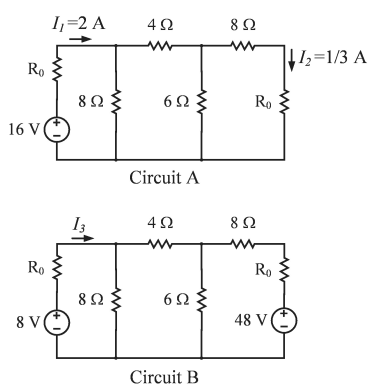
\includegraphics[width = 0.7\columnwidth]{GATE/2022/IN/figs/q54}
\caption{}
\label{fig:q54}
\end{figure}

